% ---------------------------------------------------------------------------------------------------------
% 結果 I：物理（864 条件グリッド，実験 1，実験 9）
% ---------------------------------------------------------------------------------------------------------
\section{結果 I：物理}
\label{sec:results}
\subsection{最適解の構造}
図~\ref{fig:oracle3d} に，$T=18$\,s，$m=66$\,kg，離手位相 $\phi_\ell=0.25$ の最適解を示す．
挑戦者は \refDw\,s 待ってから振り始め，\refDs\,s かけて勢いをつけ，体をほぼ一直線に伸ばして離手する．
\refDf\,s の飛行の間に体を丸めて向きを変え，B を捕捉する．
捕捉後は勢いで体が B の壁の下をくぐって前方へ振れ，振れ戻って 2\,s の保持を終える．
\begin{figure*}[t]
\centering
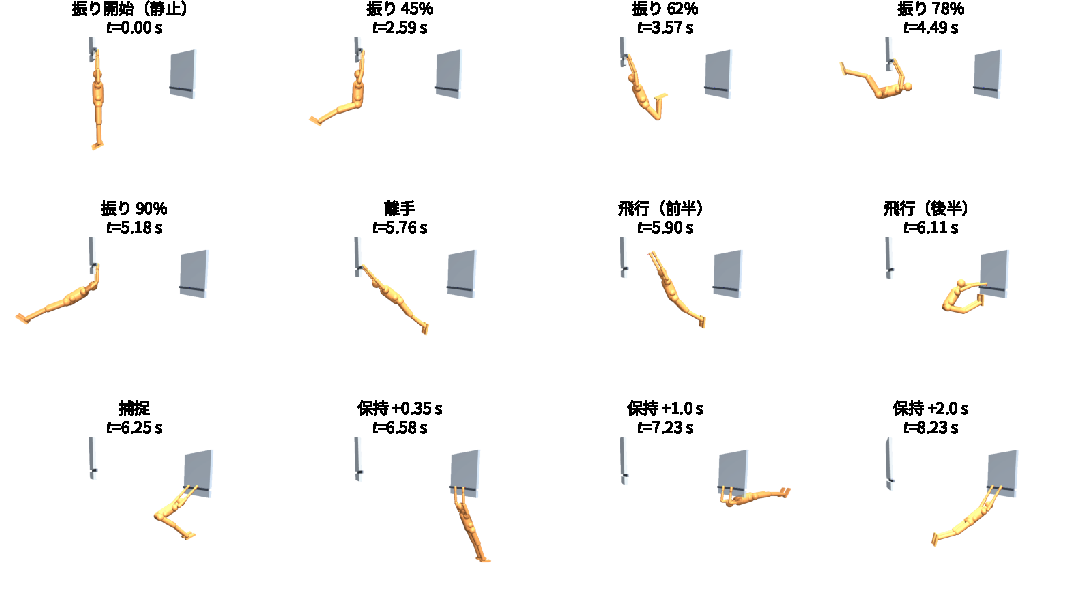
\includegraphics[width=\linewidth]{../results/figs/oracle3d.pdf}
\caption{最適解の 3 次元連続図（$T=18$\,s，$m=66$\,kg，$\phi_\ell=0.25$）．$t$ は振り開始からの時間．
各コマの装置はその時刻の位置にある（A は下降し，B は遠ざかる）．
平面モデルは体の向きの反転を空中で自由に行えるとするので，飛行の前半は A 向き，後半は B 向きで描いた．矢状面内の関節の位置はモデルの解そのものである．}
\label{fig:oracle3d}
\end{figure*}
図~\ref{fig:timeseries} は同じ解の時間履歴である．三つのことが読み取れる．
第一に，把持利用率 $U$ は振りの大部分で 0.5 程度であり，離手の直前と捕捉の直後に $\Upk=$\refUpeak に達して平らになる．
最適化は，離手の直前と保持の最初の \refHoldPlateau\,s の両方が同時に上限に触れるように負荷を配分している．
捕捉の衝撃そのものは小さい（力積を均した負荷は \refImp）．手と突起の相対速度が小さくなるように飛行を選んでいるためである．
第二に，関節トルクは離手の前に肘が上限に張り付き，保持では逆向きに張り付く．
第三に，可動域の端までの余裕と壁との隙間は，振りの間に何度も 0 になる．
最適解は可動域の端，壁，錐の境界の上を通っており，実行の誤差に対する余裕をもたない．このことが第~\ref{sec:exec}節の結果を決める．
\begin{figure*}[t]
\centering
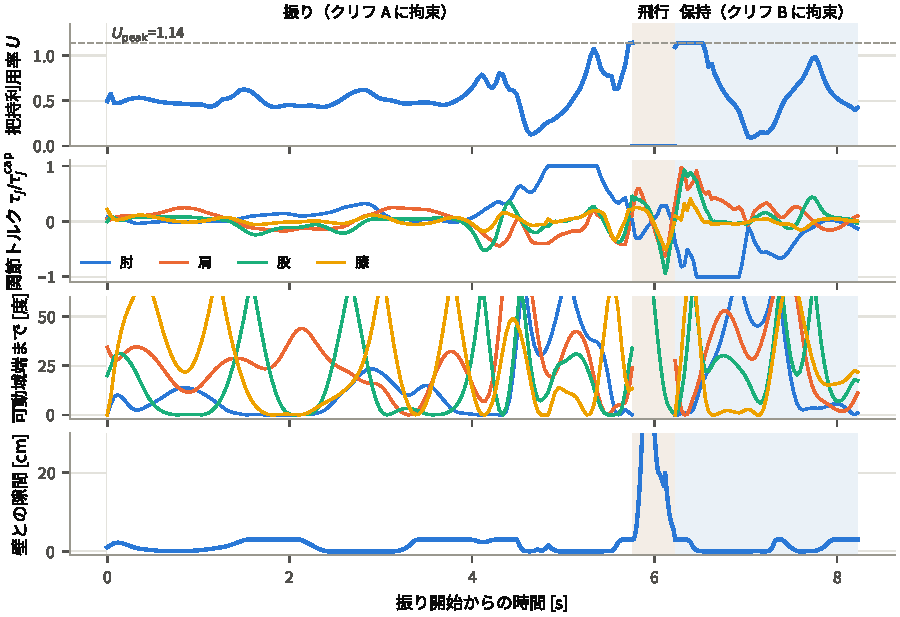
\includegraphics[width=\linewidth]{../results/figs/solution_timeseries.pdf}
\caption{図~\ref{fig:oracle3d} の解の時間履歴．上から，把持利用率 $U$（破線は $\Upk$），正規化した関節トルク，
各関節が可動域の端までどれだけ離れているか，体と壁の隙間の最小値．背景の色は相（白：振り，薄茶：飛行，薄青：保持）．}
\label{fig:timeseries}
\end{figure*}

\subsection{離手位相と必要把持容量}
\label{sec:grid}
装置周期 $T\in\{16,17,\dots,24\}$\,s，体重 $m\in\{60,63,\dots,75\}$\,kg，離手位相 $\phi_\ell\in\{0,1/16,\dots,15/16\}$ の \gridN 条件を解いた
（図~\ref{fig:grid}，図~\ref{fig:gridmap}，表~\ref{tab:grid}）．\gridNok 条件で解が収束した．
収束しなかった \gridNfail 条件（実行不可能と判定されたものが \gridInfeasible，時間または反復の上限に達したものが \gridTimeout）は，
すべて $\phi_\ell=$\phiFail にある．

\textbf{連続法の必要性．}一つの $(T,m)$ について離手位相を順に送りながら前の解を初期値にして解く方法（連鎖掃引）だけでは，
解は一度 $\Upk\approx3$ の局所解に落ちると，その後の位相でもそこから抜けられなかった．
同じ位相が隣の周期では $\Upk\approx1.1$ で解けているにもかかわらず，である．
そこで，周期・体重・位相の格子上で隣り合う条件の解を初期値にして解き直す連続法を，改善がなくなるまで繰り返した．
\polImproved 条件で解が改善し，うち \polBig 条件は $\Upk>2$ から $\Upk\le2$ へ移った．
$\Upk\le2$ の条件数は \preFeasTwo から \gridFeasTwo に増えた（図~\ref{fig:gridmap}(b)）．
連鎖掃引だけの結果では復路がほとんど実行不可能に見えたが，これは局所解によるものであった．
以下の結果は連続法を加えた後のものである．局所解である可能性は残るので，得られた $\Upk$ は必要容量の上界と読むべきである．
\begin{figure*}[t]
\centering
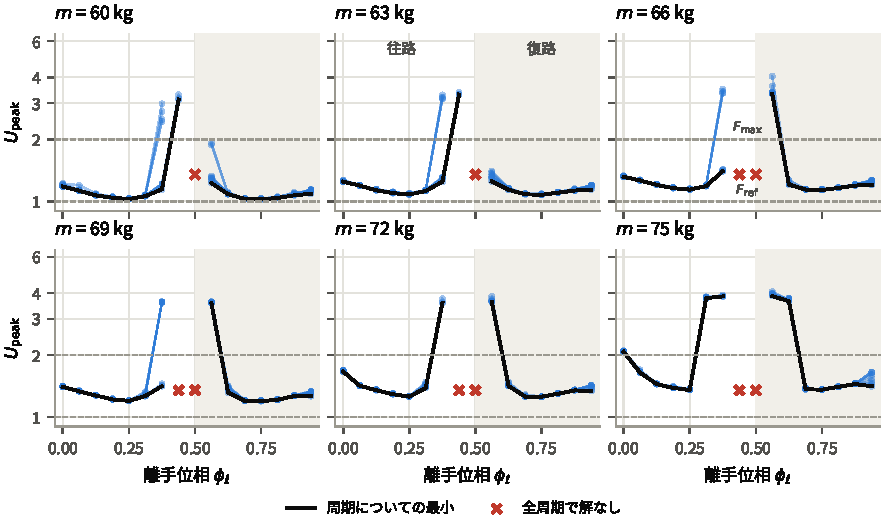
\includegraphics[width=\linewidth]{../results/figs/grid_capacity.pdf}
\caption{離手位相 $\phi_\ell$ と必要把持容量 $\Upk$（体重ごと）．細い青線は 9 通りの装置周期のそれぞれ，太い黒線は周期についての最小値．
$\times$ はどの周期でも解が得られなかった位相．破線は $\Fref$（$\Upk=1$）と見出しの許容容量 $\Fmax$（$\Upk=2$）．灰色の背景は復路．縦軸は対数．}
\label{fig:grid}
\end{figure*}
\begin{figure*}[t]
\centering
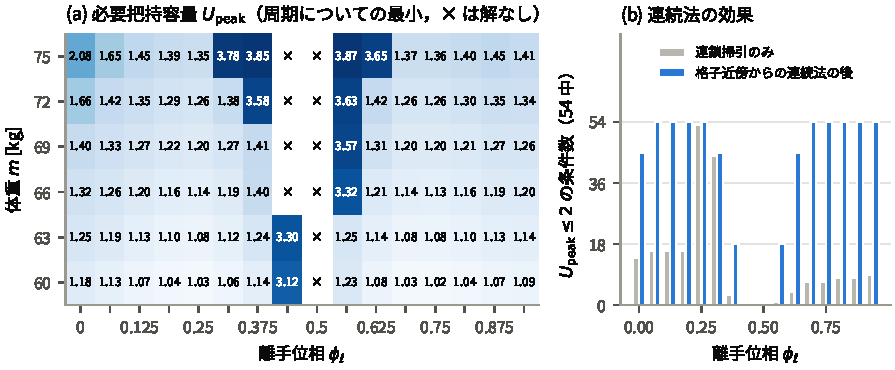
\includegraphics[width=\linewidth]{../results/figs/grid_map.pdf}
\caption{(a)~必要把持容量 $\Upk$ の地図（各体重・各離手位相について装置周期についての最小値）．
(b)~$\Upk\le2$ で解けた条件の数（各位相につき 9 周期 $\times$ 6 体重の 54 条件）．灰色は連鎖掃引だけの結果，青は格子上の連続法を加えた後．}
\label{fig:gridmap}
\end{figure*}
\begin{table*}[t]
\centering\scriptsize
\caption{体重ごとの必要把持容量（装置周期と離手位相についての最小値）と，実行可能な位相．「1.1 倍以内」は，周期についての最小値が体重ごとの最小 $\Upk$ の 1.1 倍以内に収まる離手位相の範囲．}
\label{tab:grid}
\IfFileExists{tab_grid.tex}{\resizebox{\textwidth}{!}{\begin{tabular}{rrrrrrrll}
\toprule
$m$ [kg] & 最小 $\Upk$ & 必要容量 [N] & 体重比 [BW] & 往路の最小（位相） & 復路の最小（位相） & $\Upk\le2$ の位相数 & 1.1 倍以内（往路） & 同（復路） \\
\midrule
60 & 1.024 & 1331 & 2.26 & 1.026（0.25） & 1.024（0.75） & 14/16 & 0.125〜0.3125 & 0.625〜0.9375 \\
63 & 1.076 & 1399 & 2.26 & 1.080（0.25） & 1.076（0.75） & 14/16 & 0.125〜0.3125 & 0.625〜0.9375 \\
66 & 1.135 & 1475 & 2.28 & 1.140（0.25） & 1.135（0.75） & 13/16 & 0.125〜0.3125 & 0.625〜0.9375 \\
69 & 1.196 & 1555 & 2.30 & 1.200（0.25） & 1.196（0.75） & 13/16 & 0.125〜0.3125 & 0.625〜0.9375 \\
72 & 1.257 & 1635 & 2.31 & 1.258（0.25） & 1.257（0.75） & 12/16 & 0.125〜0.25 & 0.6875〜0.9375 \\
75 & 1.354 & 1761 & 2.39 & 1.354（0.25） & 1.359（0.75） & 9/16 & 0.125〜0.25 & 0.6875〜0.9375 \\
\bottomrule
\end{tabular}
}}{（計算中）}
\end{table*}

\IfFileExists{grid_paragraph.tex}{\textbf{実行可能な位相．}見出しの許容容量 $\Upk\le2$ で解が得られる離手位相は，往路では $\phi_\ell=0.062$〜$0.25$ が全体重に共通である．
復路で $\Upk\le2$ の解が得られたのは $m=$60，63，72\,kg だけで，位相は $\phi_\ell=0.562$〜$0.938$ である．
$\phi_\ell=0.438$〜$0.5$ では，どの体重でも $\Upk\le2$ の解は得られなかった．B が最も遠い $\phi=0.5$ の前後で，先端間距離は 2.6〜2.7\,m になり，A は最も低い位置にある．片側からの振りでは，この距離を越える離手の速度と高さが得られない．

\textbf{体重と装置周期．}必要把持容量の最小値は，$m=60$\,kg の \capSixty から $m=75$\,kg の \capSeventyFive へ体重とともに増える（体重比では \capBWmin〜\capBWmax\,BW）．関節トルクの上限を体重によらず固定しているので，重い体ほど振りに使える余力が小さく，体重比でも要求が増える．装置周期への依存は小さい．$\phi_\ell=0.25$ では，9 通りの周期の間の $\Upk$ の違いは最大 \periodSpreadMax\,\%（中央値 \periodSpreadMed\,\%）である．装置の速さは 0.08〜0.11\,m/s で，離手のときの体の速さ（数 m/s）に比べて小さい．飛行時間は \flightMin〜\flightMax\,s で，その間に装置が動く距離は 5\,cm 以下である．効くのは離手の瞬間の装置の位置であって，速さではない．

\textbf{最大負荷が生じる相．}$\Upk\le2$ で解けた \gridFeasTwo 条件のうち，保持の最大負荷が $\Upk$ に達しているものは \holdAtPeak\,\%，振りの最大負荷が $\Upk$ に達しているものは \swingAtPeak\,\%である．多くの解で両方が同時に上限に触れている．どちらが必要容量を決めているかは，到達しているかどうかでは分からない．これを第~\ref{sec:interventions}節で調べる．
}{}

\subsection{目的関数の重み}
\label{sec:objective}
式~\eqref{eq:objective} の重みが結論を変えないかを，$T=18$\,s の 12 条件（3 体重 $\times$ 4 位相）で調べた（図~\ref{fig:objective}，表~\ref{tab:objective}）．
比べたのは，本稿の重み $w_U=10$，その 10 倍と 10 分の 1，$\Upk$ だけを最小化する容量最優先，
および容量最優先の最小値 $\hat U$ の 1.01 倍以内という制約のもとで努力を最小化する辞書式の 5 通りである．
$\Upk\le2$ で解けた \objNcond 条件では，本稿の重みによる $\Upk$ は容量最優先の最小値より最大 \objCurMax\,\%（中央値 \objCurMed\,\%）大きいだけである．
重みを 100 にすると差は \objWhundredMax\,\%以下になり，1 にすると最大 \objWoneMax\,\%になる．
容量最優先の解は努力が \objLexEffMin〜\objLexEffMax\,\%増える．
$w_U\ge10$ であれば，必要把持容量についての結論は重みに依らない．
\begin{figure*}[t]
\centering
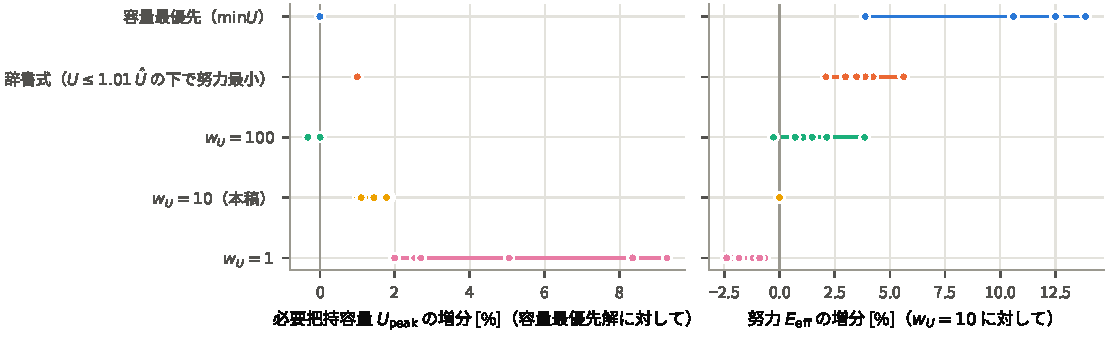
\includegraphics[width=\linewidth]{../results/figs/x1_objective.pdf}
\caption{目的関数の重みと解（実験 1）．点は $\Upk\le2$ で解けた条件のそれぞれ，線はその範囲．
左：容量最優先の解に対する $\Upk$ の増分．右：本稿の重み（$w_U=10$）の解に対する努力の増分．}
\label{fig:objective}
\end{figure*}
\begin{table*}[t]
\centering\scriptsize
\caption{目的関数ごとの必要把持容量 $\Upk$ と努力 $E$（$T=18$\,s）．---は収束しなかった条件．}
\label{tab:objective}
\IfFileExists{tab_x1.tex}{\begin{tabular}{rr|rrrrr|rrr}
\toprule
$m$ [kg] & $\phi_\ell$ & 容量最優先 & 辞書式 & $w_U{=}100$ & $w_U{=}10$ & $w_U{=}1$ & $E$：容量最優先 & $E$：$w_U{=}10$ & $E$：$w_U{=}1$ \\
\midrule
60 & 0.250 & 1.014 & 1.024 & 1.014 & 1.028 & 1.098 & 3.24 & 2.85 & 2.79 \\
60 & 0.312 & 1.050 & 1.061 & 1.050 & 1.070 & 1.077 & 3.36 & 2.98 & 2.96 \\
60 & 0.375 & 2.364 & 2.387 & 2.367 & 2.440 & 2.457 & 3.87 & 3.42 & 3.39 \\
60 & 0.750 & 1.011 & 1.022 & 1.012 & 1.029 & 1.063 & 3.13 & 2.83 & 2.76 \\
66 & 0.250 & 1.128 & 1.139 & 1.128 & 1.139 & 1.233 & 3.56 & 3.43 & 3.36 \\
66 & 0.312 & 1.182 & 1.194 & 1.178 & 1.195 & 1.205 & 4.06 & 3.61 & 3.57 \\
66 & 0.375 & 3.380 & 3.414 & 3.360 & 3.403 & 3.417 & 4.36 & 3.93 & 3.91 \\
66 & 0.750 & 3.087 & 3.118 & 3.056 & 3.149 & 3.568 & 3.97 & 3.38 & 3.35 \\
75 & 0.250 & 1.339 & 1.353 & 1.339 & 1.358 & 1.375 & 4.91 & 4.44 & 4.40 \\
75 & 0.312 & 3.739 & 3.776 & 3.737 & 3.810 & 3.912 & 5.49 & 4.58 & 4.46 \\
75 & 0.375 & 5.987 & --- & 5.986 & 5.988 & 5.988 & 5.72 & 6.10 & 6.08 \\
75 & 0.750 & 3.562 & 3.597 & 3.562 & 3.586 & 4.035 & 5.20 & 4.49 & 4.21 \\
\bottomrule
\end{tabular}
}{（計算中）}
\end{table*}

\subsection{何が必要容量を決めているか}
\label{sec:interventions}
\textbf{乗数による判定．}残り最適化問題 \dsNok 個の解で，$U(t)\le\Upk$ の乗数を相ごとに合計すると，
保持が \shareHold\,\%，捕捉が \shareCatch\,\%，振りが \shareSwing\,\%を占めた．乗数は，必要容量を決めているのが保持であることを示す．

\textbf{介入による確認．}乗数は一次の量なので，実際に制約を変えて解き直して確かめた（図~\ref{fig:interventions}(a)）．
一つの相だけ把持容量の上限を 10\,\%緩めると，保持を緩めた場合に $\Upk$ は \relHoldMin〜\relHoldMax\,\%下がる．
緩めた分（$1/1.1$ で 9.1\,\%）がほぼそのまま効いている．
振りを緩めても \relSwingMax\,\%以下，捕捉を緩めても \relCatchMax\,\%以下しか下がらない．
保持の時間を 2\,s から 0.5\,s に縮めると $\Upk$ は \holdHalfMin〜\holdHalfMax\,\%下がるが，1\,s では \holdOneMax\,\%以下，3\,s に延ばしても \holdThreeMax\,\%以下しか変わらない．
保持の負荷を決めているのは，捕捉の直後から約 1\,s の間の，振れる体を支える力である．

\textbf{関節トルク．}全関節のトルク上限を変えて解き直すと（図~\ref{fig:interventions}(b)，表~\ref{tab:capsens}），
$m=60$，66\,kg では $\Upk$ の弾性（上限が 1\,\%増えたときの $\Upk$ の変化率）は $-$\elastUmin〜$-$\elastUmax である．
筋力が 10\,\%増えても必要把持容量は 1〜2\,\%しか下がらない．
$m=75$\,kg は限界に近く，上限を 5\,\%下げると解が得られなくなる．関節ごとに見ると肘の寄与が最も大きい（$m=75$\,kg で肘だけ 5\,\%下げると $\Upk$ は \elbowHeavy\,\%増える）．
乗数から求めた感度 $\partial J^*/\partial\ln\taucap$ と，解き直しによる有限差分の比は \sensRatioMin〜\sensRatioMax であった．
乗数は感度の符号と大きさの程度を正しく与えるが，$\pm$数\,\%の変化に対する値としては 3〜5 割の誤差がある．
残り最適化問題の解での価格の統計を表~\ref{tab:prices} に示す．関節角速度の上限と捕捉速度の上限は一度も拘束的にならなかった．

\textbf{捕捉モデル．}衝撃力積を均す時間 $\Delta_c$ を 25\,ms や 100\,ms に変えても $\Upk$ の変化は \dcatchMax\,\%以下である（図~\ref{fig:interventions}(c)）．
最適解は衝撃が小さくなる捕捉を選ぶので，衝撃の見積もり方は結論に効かない．
捕捉を順応モデルに置き換えると $\Upk$ は \compVsImpactMin〜\compVsImpactMax\,\%下がる．
順応モデルの剛性を半分にすると \kHalfMin〜\kHalfMax\,\%下がり，2 倍にすると \kDoubleMin〜\kDoubleMax\,\%上がる．
必要把持容量の絶対値は捕捉のモデルに 1 割程度依存する．
\begin{figure*}[t]
\centering
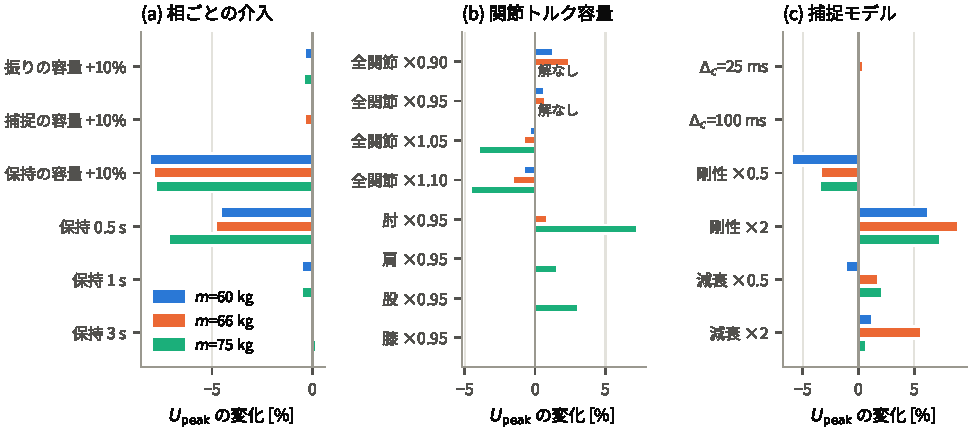
\includegraphics[width=\linewidth]{../results/figs/x9_interventions.pdf}
\caption{制約や能力を変えて解き直したときの必要把持容量の変化（実験 9；$T=18$\,s，$\phi_\ell=0.25$）．
(a)~一つの相だけ把持容量の上限を 10\,\%緩めた場合と，保持時間を変えた場合．(b)~関節トルクの上限を変えた場合．
(c)~捕捉モデルを変えた場合（$\Delta_c$ は剛体衝突モデル，剛性と減衰は順応捕捉モデルで，それぞれのモデルの基準解に対する変化）．}
\label{fig:interventions}
\end{figure*}
\begin{table}[t]
\centering\scriptsize
\caption{関節トルク上限についての感度：解き直しによる有限差分と乗数．}
\label{tab:capsens}
\IfFileExists{tab_x9sens.tex}{\resizebox{\linewidth}{!}{\begin{tabular}{lrrrr}
\toprule
$m$ [kg] & 刻み [\%] & 有限差分 $\partial J^*/\partial\ln\tau^{\rm cap}$ & 乗数 & $U_{\rm peak}$ の弾性 \\
\midrule
60 & 1 & -3.22 & -2.21 & -0.15 \\
60 & 5 & -2.64 & -2.21 & -0.11 \\
60 & 10 & -2.22 & -2.21 & -0.11 \\
66 & 1 & -2.48 & -3.41 & -0.14 \\
66 & 5 & -3.11 & -3.41 & -0.16 \\
66 & 10 & -3.71 & -3.41 & -0.20 \\
75 & 1 & -24.13 & -22.46 & -1.54 \\
\bottomrule
\end{tabular}
}}{（計算中）}
\end{table}
\begin{table*}[t]
\centering\scriptsize
\caption{能力パラメータの影の価格 $\partial J^*/\partial\ln p$（残り最適化問題 \dsNok 個の解）．弾性は $J^*$ で割った値．}
\label{tab:prices}
\IfFileExists{tab_prices2.tex}{\begin{tabular}{lrrrrr}
\toprule
パラメータ $p$ & $\partial J^*/\partial\ln p$ 中央値 & 平均 & 10\%点 & 弾性（中央値） & 拘束的な割合 [\%] \\
\midrule
関節トルク容量 $\tau^{\rm cap}$ & -4.212 & -11.416 & -26.832 & -0.288 & 100 \\
引っ掛かり係数 $\mu_{\rm out}$ & -0.183 & -0.483 & -1.348 & -0.013 & 99 \\
摩擦係数 $\mu_{\rm in}$ & -0.021 & -0.072 & -0.103 & -0.001 & 100 \\
関節角速度上限 $\dot q_{\max}$ & 0.000 & 0.000 & 0.000 & 0.000 & 0 \\
捕捉相対速度上限 $v_{\rm rel}^{\max}$ & 0.000 & 0.000 & 0.000 & 0.000 & 0 \\
壁から離れる速度上限 $v_{\rm away}^{\max}$ & 0.000 & 0.000 & 0.000 & 0.000 & 0 \\
\bottomrule
\end{tabular}
}{（計算中）}
\end{table*}
